\begin{figure}[h] 
\centering 
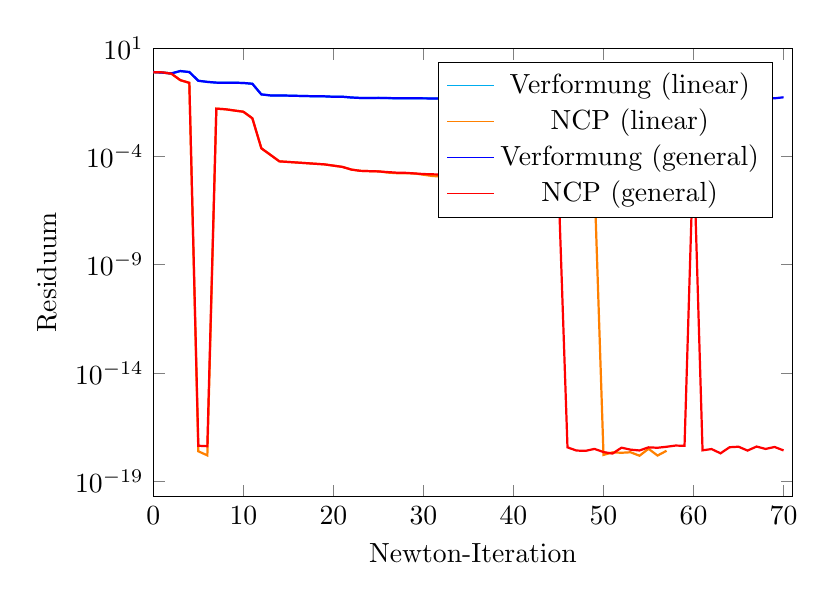
\begin{tikzpicture}[every plot/.append style={thick}] 
\begin{axis}[ 
label style={font=\normalsize}, 
xlabel={Newton-Iteration}, 
ylabel={Residuum}, 
xmin=0, xmax=71, 
ymode=log, 
ymin=0, ymax=10, 
width=0.8\textwidth, 
height=0.6\textwidth, 
legend pos=north east, 
legend style={cells={align=left}}, 
grid style=dashed, 
] 
\addplot[ 
color=cyan, 
] 
coordinates { 
(0, 7.91e-01)(1, 7.42e-01)(2, 6.82e-01)(3, 8.78e-01)(4, 7.89e-01)(5, 3.12e-01)(6, 2.77e-01)(7, 2.56e-01)(8, 2.50e-01)(9, 2.53e-01)(10, 2.47e-01)(11, 2.27e-01)(12, 7.31e-02)(13, 6.58e-02)(14, 6.58e-02)(15, 6.42e-02)(16, 6.27e-02)(17, 6.14e-02)(18, 5.99e-02)(19, 5.96e-02)(20, 5.70e-02)(21, 5.72e-02)(22, 5.26e-02)(23, 5.02e-02)(24, 4.96e-02)(25, 5.08e-02)(26, 4.93e-02)(27, 4.82e-02)(28, 4.80e-02)(29, 4.90e-02)(30, 4.88e-02)(31, 4.72e-02)(32, 4.71e-02)(33, 4.67e-02)(34, 4.69e-02)(35, 4.58e-02)(36, 4.60e-02)(37, 4.60e-02)(38, 4.57e-02)(39, 4.55e-02)(40, 4.61e-02)(41, 4.60e-02)(42, 4.55e-02)(43, 4.51e-02)(44, 4.51e-02)(45, 4.51e-02)(46, 4.50e-02)(47, 4.51e-02)(48, 4.48e-02)(49, 6.37e-02)(50, 4.22e-02)(51, 4.11e-02)(52, 4.11e-02)(53, 4.02e-02)(54, 4.14e-02)(55, 4.04e-02)(56, 4.72e-02)(57, 4.16e-02)}; 
\addlegendentry{Verformung (linear)} 
\addplot[ 
color=orange, 
] 
coordinates { 
(0, 7.80e-01)(1, 7.61e-01)(2, 6.66e-01)(3, 3.33e-01)(4, 2.50e-01)(5, 2.42e-18)(6, 1.57e-18)(7, 1.61e-02)(8, 1.51e-02)(9, 1.32e-02)(10, 1.16e-02)(11, 5.79e-03)(12, 2.37e-04)(13, 1.19e-04)(14, 5.93e-05)(15, 5.56e-05)(16, 5.21e-05)(17, 4.89e-05)(18, 4.58e-05)(19, 4.30e-05)(20, 3.76e-05)(21, 3.29e-05)(22, 2.47e-05)(23, 2.16e-05)(24, 2.09e-05)(25, 2.06e-05)(26, 1.80e-05)(27, 1.69e-05)(28, 1.66e-05)(29, 1.64e-05)(30, 1.43e-05)(31, 1.25e-05)(32, 1.18e-05)(33, 1.10e-05)(34, 1.03e-05)(35, 9.68e-06)(36, 9.53e-06)(37, 9.24e-06)(38, 8.95e-06)(39, 8.81e-06)(40, 8.67e-06)(41, 8.13e-06)(42, 7.62e-06)(43, 7.38e-06)(44, 7.27e-06)(45, 7.16e-06)(46, 7.04e-06)(47, 6.94e-06)(48, 6.83e-06)(49, 6.72e-06)(50, 1.65e-18)(51, 2.16e-18)(52, 2.07e-18)(53, 2.18e-18)(54, 1.51e-18)(55, 3.16e-18)(56, 1.54e-18)(57, 2.55e-18)}; 
\addlegendentry{NCP (linear)} 
\addplot[ 
color=blue, 
] 
coordinates { 
(0, 7.91e-01)(1, 7.42e-01)(2, 6.82e-01)(3, 8.78e-01)(4, 7.89e-01)(5, 3.12e-01)(6, 2.77e-01)(7, 2.56e-01)(8, 2.50e-01)(9, 2.53e-01)(10, 2.47e-01)(11, 2.27e-01)(12, 7.31e-02)(13, 6.58e-02)(14, 6.58e-02)(15, 6.42e-02)(16, 6.27e-02)(17, 6.14e-02)(18, 5.99e-02)(19, 5.96e-02)(20, 5.70e-02)(21, 5.71e-02)(22, 5.27e-02)(23, 5.01e-02)(24, 4.98e-02)(25, 4.98e-02)(26, 4.99e-02)(27, 4.86e-02)(28, 4.90e-02)(29, 4.88e-02)(30, 4.80e-02)(31, 4.77e-02)(32, 4.75e-02)(33, 4.86e-02)(34, 4.80e-02)(35, 4.77e-02)(36, 4.64e-02)(37, 4.59e-02)(38, 4.54e-02)(39, 4.66e-02)(40, 4.62e-02)(41, 4.62e-02)(42, 4.50e-02)(43, 4.48e-02)(44, 4.42e-02)(45, 5.87e-02)(46, 4.70e-02)(47, 4.60e-02)(48, 4.20e-02)(49, 4.17e-02)(50, 4.20e-02)(51, 4.19e-02)(52, 4.18e-02)(53, 4.23e-02)(54, 4.17e-02)(55, 5.13e-02)(56, 4.13e-02)(57, 4.08e-02)(58, 4.73e-02)(59, 4.19e-02)(60, 1.57e-01)(61, 8.86e-02)(62, 8.76e-02)(63, 8.74e-02)(64, 8.03e-02)(65, 5.45e-02)(66, 5.47e-02)(67, 4.89e-02)(68, 4.86e-02)(69, 4.83e-02)(70, 5.39e-02)}; 
\addlegendentry{Verformung (general)} 
\addplot[ 
color=red, 
] 
coordinates { 
(0, 7.80e-01)(1, 7.61e-01)(2, 6.66e-01)(3, 3.33e-01)(4, 2.50e-01)(5, 4.36e-18)(6, 4.16e-18)(7, 1.61e-02)(8, 1.51e-02)(9, 1.32e-02)(10, 1.16e-02)(11, 5.79e-03)(12, 2.37e-04)(13, 1.19e-04)(14, 5.93e-05)(15, 5.56e-05)(16, 5.21e-05)(17, 4.89e-05)(18, 4.58e-05)(19, 4.30e-05)(20, 3.76e-05)(21, 3.29e-05)(22, 2.47e-05)(23, 2.16e-05)(24, 2.09e-05)(25, 2.03e-05)(26, 1.90e-05)(27, 1.78e-05)(28, 1.75e-05)(29, 1.64e-05)(30, 1.54e-05)(31, 1.49e-05)(32, 1.47e-05)(33, 1.45e-05)(34, 1.27e-05)(35, 1.11e-05)(36, 9.69e-06)(37, 9.09e-06)(38, 8.80e-06)(39, 8.67e-06)(40, 7.58e-06)(41, 6.64e-06)(42, 5.81e-06)(43, 5.44e-06)(44, 5.27e-06)(45, 5.19e-06)(46, 3.67e-18)(47, 2.62e-18)(48, 2.53e-18)(49, 3.12e-18)(50, 2.23e-18)(51, 1.90e-18)(52, 3.55e-18)(53, 2.88e-18)(54, 2.64e-18)(55, 3.68e-18)(56, 3.52e-18)(57, 3.91e-18)(58, 4.45e-18)(59, 4.34e-18)(60, 2.56e-04)(61, 2.68e-18)(62, 3.07e-18)(63, 1.95e-18)(64, 3.73e-18)(65, 3.93e-18)(66, 2.61e-18)(67, 4.01e-18)(68, 3.11e-18)(69, 3.83e-18)(70, 2.65e-18)}; 
\addlegendentry{NCP (general)} 
\end{axis} 
\end{tikzpicture} 
\caption{Residuen des Stoffgesetzes 'St.Venant' mit Hinderniss 'Spitze' und 2178 Freiheitsgraden für die Verschiebung.} 
\label{fiq:St.Venant_Spitze_level4} 
\end{figure} 
